%!TEX root = ../../main.tex

% Processo de aprendizado
% Tarefa de classificação binária
% Divisão dos Dados
% Explicação do método holdout
% Parâmetros e hiperparâmetros
% Métricas Utilizadas - cenários balanceados e desbalanceados

A tarefa de aprendizado disposta neste trabalho consiste em uma tarefa de classificação binária, ou seja, a sua saída possui apenas dois valores possíveis.


\begin{figure}[h!]
\centering
\caption{Uma visão geral do processo de aprendizado.}
\label{fig:esquema-solucao}
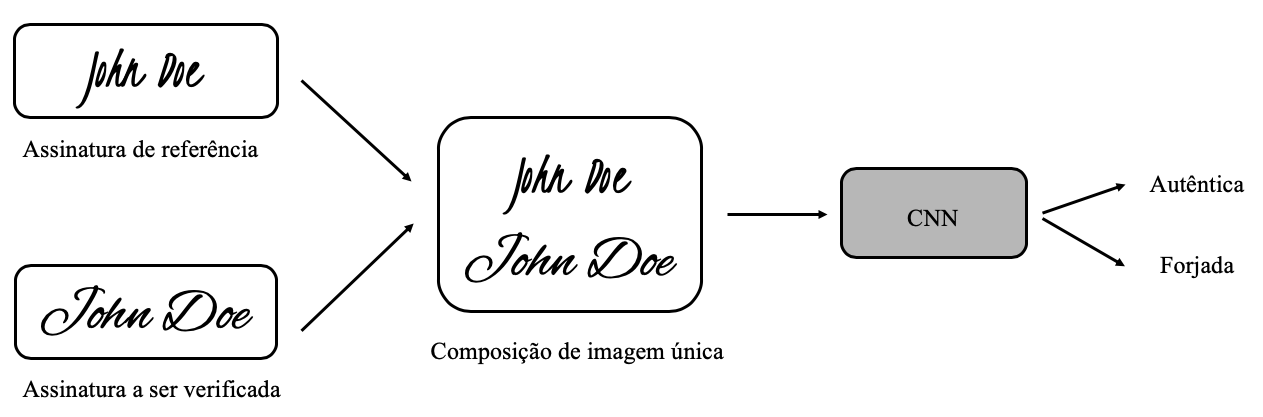
\includegraphics[width=\textwidth]{imgs/esquema-solucao}
\end{figure}

O treinamento e testes das CNNs seguirão o comportamento \emph{holdout} de validação
cruzada, em que $70\%$ dos dados serão utilizados no treino e ajuste de parâmetros e o
restante para avaliação, com vista a capturar a qualidade da generalização proposta pelos
modelos considerados.
